\begin{figure}[H]
  \centering
  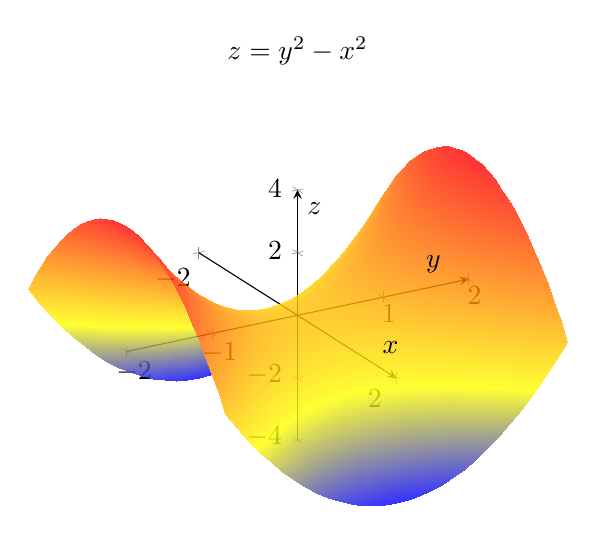
\begin{tikzpicture}
    \begin{axis}[
      view={60}{30},
      axis lines=middle,
      xlabel={$x$},
      ylabel={$y$},
      zlabel={$z$},
      domain=-2:2,
      y domain=-2:2,
      samples=31,
      mesh/ordering=y varies,
      z buffer=sort,
      grid=major,
      title={$z = y^2 - x^2$}
    ]
      \addplot3[
        surf,
        shader=interp,
        opacity=0.8
      ]
      {y^2 - x^2};
    \end{axis}
  \end{tikzpicture}
  \caption{Superfície $z = y^2 - x^2$ (parabolóide hiperbólico).}
\end{figure}

\subsection{Hiperbolóide cilinfrico.}
\begin{figure}[H]
  \centering
  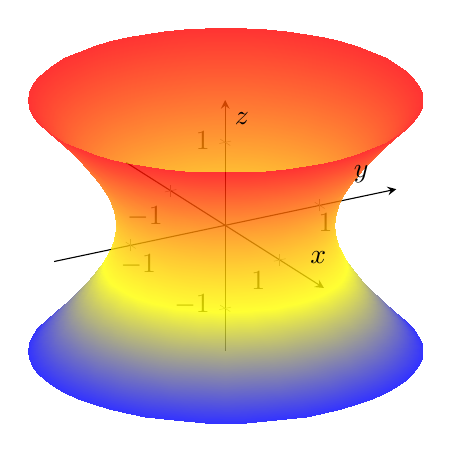
\begin{tikzpicture}
    \begin{axis}[
      view={60}{30},
      axis lines=middle,
      xlabel={$x$},
      ylabel={$y$},
      zlabel={$z$},
      domain=0:360,          % u em graus
      y domain=-1.2:1.2,     % v (faixa controla "altura"/abertura)
      samples=61,
      samples y=31,
      z buffer=sort,
      grid=major,
      mesh/ordering=y varies
    ]
      \addplot3[
        surf,
        shader=interp,
        opacity=0.8
      ]
      (
        {cosh(y)*cos(x)},
        {cosh(y)*sin(x)},
        {sinh(y)}
      );
    \end{axis}
  \end{tikzpicture}
\end{figure}
\subsection{como se fossem 2 cones}

\subsection{Hiperbolóide cilinfrico.}
\begin{figure}[H]
  \centering
  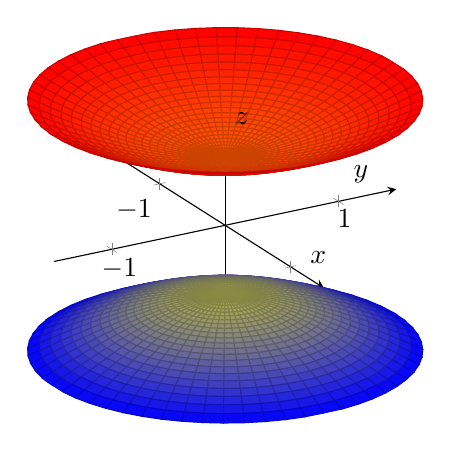
\begin{tikzpicture}
    \begin{axis}[
      view={60}{30},
      axis lines=middle,
      xlabel={$x$},
      ylabel={$y$},
      zlabel={$z$},
      domain=0:360,          % u em graus
      y domain=-1.2:1.2,     % v (faixa controla "altura"/abertura)
      samples=61,
      samples y=31,
      z buffer=sort,
      grid=major,
      mesh/ordering=y varies
    ]
% folha de cima
\addplot3[surf, samples=60, samples y=25, domain=0:360, y domain=0:1.2]
(
  {sinh(y)*cos(x)},  % x = sinh(u) cos(v)
  {sinh(y)*sin(x)},  % y = sinh(u) sin(v)
  {cosh(y)}          % z = +cosh(u)  (a=1)
);

% folha de baixo
\addplot3[surf, samples=60, samples y=25, domain=0:360, y domain=0:1.2]
(
  {sinh(y)*cos(x)},
  {sinh(y)*sin(x)},
  {-cosh(y)}         % z = -cosh(u)
);

    \end{axis}
  \end{tikzpicture}
\end{figure}
\subsection{Hiperbolóide}

\begin{figure}[H]
  \centering
  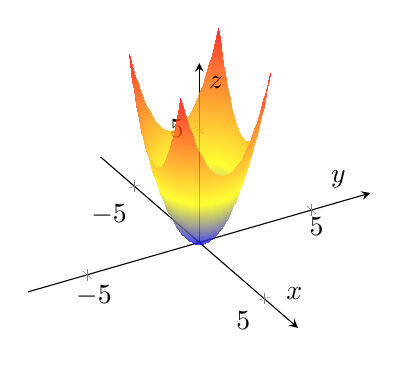
\begin{tikzpicture}
    \begin{axis}[
      view={60}{30},
      axis lines=middle,
      xlabel={$x$}, ylabel={$y$}, zlabel={$z$},
      domain=-2:2,
      y domain=-2:2,
      samples=41,
      samples y=41,
      z buffer=sort,
      grid=major,
      axis equal,                 % ajuda a “não distorcer” a forma
      title={},
    ]
      \addplot3[
        surf,
        shader=interp,
        opacity=0.8
      ]
      {x^2 + y^2};                % <-- “sino”
    \end{axis}
  \end{tikzpicture}
  \caption{}
\end{figure}